% !TeX program = xelatex
%% SEEP2026 proceedings - 6-page extended-abstract (short) version.
%% Condensed from MAIN.tex. Compile with XeLaTeX (real Arial / Arial Narrow /
%% Times New Roman required by the template). It will NOT compile with pdfLaTeX.
\documentclass[12pt,a4paper]{article}

% ---------- Type area ----------
\usepackage[a4paper,top=2cm,bottom=2cm,left=2.5cm,right=2.5cm,%
            headsep=0.6cm,includehead]{geometry}

% ---------- Math ----------
\usepackage{amsmath}

% ---------- Fonts (template-specified) ----------
\usepackage{fontspec}
\setmainfont{Times New Roman}                 % Body text, affiliation, header
\newfontfamily\arialfont{Arial}               % Headings, authors, captions
\newfontfamily\arialnarrow{Arial Narrow}      % Paper title

% Times-consistent math (digits, upright and symbols), integrated with fontspec.
% Replaces newtxmath, which under XeLaTeX let math digits fall back to Latin Modern.
\usepackage{unicode-math}
\setmathfont{texgyretermes-math.otf}          % Times-clone math font

% ---------- Graphics ----------
\usepackage{graphicx}
\usepackage{subcaption}

% ---------- Running header (every page), no page numbers ----------
\usepackage{fancyhdr}
\newcommand{\seepheader}{\itshape Proceedings of SEEP2026, 20-23 July 2026,%
\ Tor Vergata University, Rome, Italy}
\pagestyle{fancy}
\fancyhf{}
\setlength{\headheight}{14.5pt}
\renewcommand{\headrulewidth}{0pt}
\fancyhead[L]{\normalfont\fontsize{12}{14}\selectfont\seepheader}
\fancypagestyle{plain}{%
  \fancyhf{}%
  \renewcommand{\headrulewidth}{0pt}%
  \fancyhead[L]{\normalfont\fontsize{12}{14}\selectfont\seepheader}%
}
\pagenumbering{gobble}            % no page numbers

% ---------- Section headings (Heading 1/2/3 styles) ----------
\usepackage{titlesec}
\setcounter{secnumdepth}{2}       % third-order headings are NOT numbered

% Heading 1: Arial, bold, 12pt, ALL CAPS, left, numbered
\titleformat{\section}
  {\arialfont\bfseries\fontsize{12}{14}\selectfont}
  {\thesection}{0.8em}{\MakeUppercase}
% Heading 2: Arial, bold, 12pt, left, numbered
\titleformat{\subsection}
  {\arialfont\bfseries\fontsize{12}{14}\selectfont}
  {\thesubsection}{0.8em}{}
% Heading 3: Arial, italic, 12pt, left, NOT numbered
\titleformat{\subsubsection}
  {\arialfont\itshape\fontsize{12}{14}\selectfont}
  {}{0pt}{}
\titlespacing*{\section}      {0pt}{8pt}{4pt}
\titlespacing*{\subsection}   {0pt}{6pt}{3pt}
\titlespacing*{\subsubsection}{0pt}{5pt}{2pt}

% ---------- Captions (Figure/Table Heading: Arial, 12pt, centered, per template) ----------
\usepackage{caption}
\DeclareCaptionFont{arial}{\arialfont\fontsize{12}{14}\selectfont}
\captionsetup{font=arial,labelfont=arial,labelsep=period,%
              justification=centering,singlelinecheck=true}

% ---------- Abstract: "ABSTRACT" centered, bold, Arial ----------
\renewenvironment{abstract}{%
  \begin{center}%
    {\arialfont\bfseries\fontsize{12}{14}\selectfont ABSTRACT}%
  \end{center}%
  \par\noindent\ignorespaces
}{\par\vspace{6pt}}

% ---------- Keywords command ----------
\newcommand{\keywords}[1]{\par\noindent{\itshape Keywords}: #1\par\vspace{6pt}}

\begin{document}

%%% TITLE, AUTHORS, AFFILIATION (Title block per SEEP2026 template)
\begin{center}
  {\arialnarrow\bfseries\fontsize{14}{17}\selectfont
   \MakeUppercase{CFD-ML-Based Turbulence Model Definition for Fidelity
   Improvement of Horizontal-Axis Wind Turbine RANS Simulations}\par}
  \vspace{6pt}
  {\arialfont\bfseries\fontsize{12}{14}\selectfont Andrea Carloni\textsuperscript{1}, Giovanni Delibra\textsuperscript{2}, Filippo De Girolamo\textsuperscript{3}, Lorenzo Tieghi\textsuperscript{4}, Alessandro Corsini\textsuperscript{2}, Valerio Francesco Barnabei\textsuperscript{2}\par}
  \vspace{2pt}
  {\fontsize{12}{14}\selectfont
   1.\ Department of Electrical and Energy Engineering, Sapienza University
   of Rome, Italy; email: andrea.carloni@uniroma1.it\par}
  {\fontsize{12}{14}\selectfont
   2.\ Department of Mechanical and Aerospace Engineering, Sapienza University
   of Rome, Italy;}
  {\fontsize{12}{14}\selectfont
   3.\ Division of Fluid Mechanics, KTH Royal Institute of Technology, Stockholm, Sweden;}
  {\fontsize{12}{14}\selectfont
   4.\ Department of Civil, Environmental and Mechanical Engineering, University of Trento, Trento, Italy;}
\end{center}
\vspace{6pt}

%%% ABSTRACT
\begin{abstract}
Accurate prediction of horizontal-axis wind turbine (HAWT) wakes is essential
for wind farm design, yet affordable tools struggle: Large Eddy Simulation (LES)
is reliable but prohibitively expensive, while unsteady RANS (URANS)
systematically mis-predicts the wake recovery. This work uses machine learning to define, rather than post-process, a machine learning-based turbulence closure of a $k$-$\omega$ SST RANS solver for HAWT wakes. From a single high-fidelity LES of the NREL-5MW turbine in a turbulent atmospheric boundary layer (ABL), an LES-equivalent eddy viscosity $\nu_{t,eq}$ is extracted as target; a K-means clustering segments the flow and a Multi-Layer Perceptron (MLP) learns the local correction $\Delta\nu_t = \nu_{t,eq} - \nu_{t,\mathrm{RANS}}$. The machine learning models and correction is thend embedded into a modified OpenFOAM PIMPLE solver. By design the closure is calibrated on this single case and transferred without retraining to unseen grids and inflow velocities, the core premise of the method. The network reproduces $\nu_{t,eq}$ with a validation $R^2 = 0.9952$; once embedded, the ML-RANS model outperforms the standard $k$-$\omega$ SST model in near- and far-wake and, most notably, on ultra-coarse grids captures the post-breakdown recovery at a cost about $1.25$ times lower than the reference LES, while also reproducing the rotor forces and power coefficients.
\end{abstract}

\keywords{Wind turbine wake, URANS, Machine learning, Turbulence modelling}

%%% INTRODUCTION
\section{Introduction}
\label{sec:introduction}
Wind energy is a cornerstone of the transition toward sustainable electricity
generation. Turbines' rotor interactions with the upcoming wind flow generates low-speed, high turbulence wakes, which are characterised by multi-scale phenomena both in terms of space and time; downstream turbines operating within it suffer reduced power output and increased fatigue loads~\cite{Porte-Agel2020}, so accurate wake prediction is essential for wind farm layout optimisation, energy-yield estimation and load assessment. Furthermore, wakes behaviour is deeply coupled with the atmospheric boundary layer (ABL), whose recovery is governed by shear-driven turbulent mixing~\cite{Porte-Agel2020}, site topology and surface roughness. Available modelling strategies trade fidelity against cost: analytical wake models are near-instantaneous but stronglysimplified; LES resolves the dominant structures but can demand $10^5$--$3\times10^6$ CPU hours per wind farm~\cite{Steiner2021}; URANS is about two orders of magnitude cheaper~\cite{Steiner2021}, but its closure assumptions cause a systematic mis-prediction of the wake recovery~\cite{72116acdc5aa4b3b8fc752f1b2fa9958}.

Machine learning (ML) is increasingly used in wind energy, most often downstream of a physical model for power forecasting or layout optimisation, leaving the turbulence model unchanged~\cite{GholamiAnjiraki2025}. A more recent line corrects or replaces the closure itself during the simulation~\cite{Duraisamy2019,Ling2016}; in the wind-energy context, corrective fields derived from time-averaged LES data have produced improved RANS wake predictions~\cite{Steiner2021,King_2018}.

This work contributes in that framework in three ways: a K-means clustering segments the domain into physically distinct regions~\cite{Clustering_tieghi,Carloni2026}, moving the correction from a cell-wise to a region-wise basis that is more interpretable, less mesh-sensitive and embedd higher generalizability; a MLP learns the local cluster-based correction $\Delta\nu_t = \nu_{t,eq} - \nu_{t,\mathrm{RANS}}$, embedded directly into the OpenFOAM PIMPLE solver so that it actively drives the momentum equations rather than being applied a posteriori.
Crucially, the closure is deliberately trained on a single reference case and transferred without retraining to coarser grids and unseen inflow velocities: this single-case-to-many transfer is the design target of the method, not a data-scarcity workaround, and is shown to deliver LES-time-averaged-like wake representation at a cost lower than standard LES. In essence, ML is used here to define the turbulence model, within the scalar eddy-viscosity framework for direct solver embedding, rather than to post-process its output.

%%% METHODOLOGY
\section{Methodology}
\label{sec:methodology}
The methodology combines a CFD part, used to generate the data and to test the
model, and an ML part, used to train the clustering and neural-network models.

\subsection{CFD dataset}
Simulations are performed with OpenFOAM-v22.12 using an in-house Actuator Line
Model (ALM)~\cite{10.1115/1.1471361} based on the \textit{turbinesFoam}
library~\cite{turbinesFoam}, under incompressible flow conditions, solving
$\vec{U}$ and $p$ with the PIMPLE algorithm. RANS simulations use the
$k$-$\omega$ SST model~\cite{doi:10.2514/3.12149}; LES uses the WALE
model~\cite{WALE}.A logarithmic velocity profile is imposed at the inlet;
at the LES inlet, synthetic turbulent fluctuations from the Kaimal
spectrum~\cite{kaimal} are superimposed following~\cite{Davidson2007UsingIS,Carloni2026}.

To generate the regression data, a modified RANS run imports the mean $\vec{U}$ and $p$ fields from the LES and, fixing those fields, performs a single step in which the $\nu_t$ field is solved consistently with the LES input inside the turbulence correction loop, yielding the modified eddy viscosity $\nu_{t,mod}$. The computational domain is a rectangular box with the rotor at 5$D$ from the inlet, 15$D$ from the outlet and 90~m from the terrain, extending 5$D$ on each side and 8$D$ in the vertical direction. The finest mesh has $\sim$30.8~M cells (minimum cell size 1.75~m near the rotor). Coarser grids of $\sim$15.9, $\sim$9.1 and $\sim$4.2~M cells are obtained by varying the domain subdivision with same relative-to-max-cell-size refinement, and are used to assess the mesh-refinement influence on the trained models.

\subsection{LES-equivalent eddy viscosity and ML target}
Here $\nu_t$ denotes the kinematic turbulent viscosity entering the RANS equations through the effective viscosity $\nu_{eff} = \nu + \nu_t$. The reference LES equivalent eddy viscosity $\nu_{t,eq}$ is obtained by projecting the deviatoric part of the LES turbulent stress (sum of resolved and subgrid-scale contributions) onto the Boussinesq form, $\Sigma_{ij}^{dev} \simeq -2\,\nu_{t,eq}\,S_{ij}$. Assuming a Smagorinsky-type subgrid stress $\tau_{ij}^{sgs,dev} = -2\,\nu_{sgs}\,S_{ij}$ and minimising the Frobenius norm of the residual gives the closed form 
\begin{equation}
    \nu_{t,eq} = \nu_{sgs}
    - \frac{\left(R_{ij}^{res}\right)^{dev} S_{ij}}{2\,S_{ij}S_{ij}} ,
\end{equation}
where $S_{ij}$ is the resolved strain-rate tensor and $R_{ij}^{res}$ the resolved Reynolds stress tensor. By construction this is the scalar eddy viscosity that best matches the deviatoric LES stress in a least-squares sense; it deliberately discards the Reynolds-stress anisotropy in exchange for direct compatibility with a standard eddy-viscosity solver. Rather than predicting $\nu_{t,eq}$ directly, the network is trained on the discrepancy with respect to the RANS baseline,
\begin{equation}
    \Delta\nu_t = \nu_{t,eq} - \nu_{t,\mathrm{RANS}} ,
    \qquad
    \nu_{t,ML} = \nu_{t,\mathrm{RANS}} + \Delta\nu_{t,ML} .
\end{equation}

\subsection{Clustering and neural network}
A K-means clustering algorithm~\cite{Carloni2026,Clustering_tieghi}, implemented in \textit{scikit-learn}~\cite{scikit-learn}, identifies the distinct flow regions of the wake, moving the prediction from a cell-wise to a region-aware basis that is more robust to mesh refinement and embedd higher generalizability. The algorithm minimises the within-cluster sum of squares, $\sum_{i=1}^{K}\sum_{x_j\in C_i}\lVert x_j-\mu_i\rVert^2$, and the optimal number of clusters $K$ is selected with the elbow method. Features are Min-Max normalised and projected on a cylindrical reference system centred on the rotor and aligned with the rotor axis; a subset of features is retained based on PCA and physical reasoning.

The regression model is a MLP implemented in TensorFlow-Keras~\cite{tensorflow2015-whitepaper}, with a single scalar output $\Delta\nu_{t,ML}$. The cell-level input vector includes $\vec{U}_{cyl}$, $k$, $\nu_{t,\mathrm{RANS}}$, the distance from the assigned cluster centroid in features space, the non-dimensional coordinates $z/D$ and $x/D$, and the (one-hot encoded) cluster labels; continuous features and the target are normalised with Standard scaler algorithm. The architecture is a sequence of fully connected residual blocks (Dense layer with L2 regularisation, Layer Normalization, GELU activation and Dropout) with progressively decreasing widths, trained by minimising a weighted Huber loss with the Adam optimizer; sample weights compensate for cluster imbalance and emphasise downstream wake samples. After a first standard $k$-$\omega$ SST iteration, the clustering assigns a cluster to each cell and the MLP predicts $\nu_{t,ML}$, which is then used to advance $\vec{U}$ and $p$ in the modified PIMPLE turbulence correction loop; the procedure is repeated every iteration. Only the eddy viscosity entering the momentum equations is replaced, while $k$ and $\omega$ retain the standard SST transport and its boundedness treatment; the solver remained stable on all grids and inflow conditions, with no LES data used at run time.

%%% CASE STUDY
\section{Case study}
\label{sec:case_study}
The methodology is tested on the NREL-5MW~\cite{NREL_5MW} HAWT, modelled with the ALM with the number of nodes adapted to each grid so that $\epsilon \le 2\Delta x$ and $\Delta b/\Delta x \le 0.5$~\cite{inproceedings}. A hub-height ($90$~m) inflow velocity $U_{ref} = 11.4\,\mathrm{m/s}$ is considered as the reference (training) condition, with two further inflow velocities of $8$ and $15\,\mathrm{m/s}$ used to assess generalization; the ABL logarithmic profile reads
\begin{equation}
    U(z) = U_{ref}\,\frac{\ln\!\big((z+z_0)/z_0\big)}{\ln\!\big((z_{ref}+z_0)/z_0\big)} .
    \label{eq:ABL_log_equation}
\end{equation}
The CFD dataset was validated against literature results~\cite{alessio5-mw,Troldborg} as in~\cite{Carloni2026} and is omitted here for brevity. Training data are sampled along two planes through the rotor centre (one parallel and one perpendicular to the terrain) on the finest grid, yielding $\sim$180k cells; the far-upstream inflow region ($x/D<-2.5$) is excluded, retaining $\sim$160k cells split 80/20 into training and validation sets, stratified by cluster.

%%%TODO: controlla bene e riscrivi i risultati quando li avrai
%%% RESULTS
\section{Results}
\label{sec:results}
The clustering identifies a clear elbow at $K=7$, separating the undisturbed flow from the inlet/ABL-affected, near-wake, mixing/breakdown and far-wake regions, consistently with the underlying physics as in previous work ~\cite{Carloni2026}. Trained in $\sim$0.24~s, it provides the region labels used by the network.

The MLP (trained at $U_\infty = 11.4\,\mathrm{m/s}$) reaches its best checkpoint at epoch 220. In physical space the reconstructed field attains $R^2 = 0.9954$ on training and $R^2 = 0.9952$ ($RMSE = 0.2635$, $MAE = 0.1797$) on validation. A residual underestimation bias persists only in the inlet region, where the synthetic boundary condition introduces numerical instabilities. An equivalent network trained without clustering attains slightly worse metrics across the board ($R^2 = 0.9950$, with higher $RMSE$/$MAE$). This aggregate gap is small only because the metrics are dominated by the large free-stream region; the benefit of clustering is concentrated in the near-terrain region, where the clustered model is markedly more consistent with the LES reference, and in the interpretability and case- and mesh-robustness it adds.

The trained model is embedded in the RANS solver and evaluated across grids of different resolution. As shown in Fig.~\ref{fig:velocity_deficit}, on the fine grid ($\sim$15.9~M cells) the ML-RANS model consistently outperforms the standard RANS model, especially in the upper near-wake where the standard model underestimates the deficit; a moderate underestimation persists in the lower near-wake, while the far-wake (after breakdown, from $4D$) is slightly overestimated. The most relevant result is obtained on the ultra-coarse grids: the model retains its improved near-wake prediction while also providing a much more accurate far-wake, including the post-breakdown recovery that is critical to estimate the power production of downstream turbines. This is achieved at a reduced cost: on the $\sim$4.2~M cells grid the ML-RANS model is about $1.25$ times cheaper than the reference LES, making it a viable tool for large-scale wind farm simulations.

Consistently with its single-case-to-many premise, the closure transfers to the
unseen $8$ and $15\,\mathrm{m/s}$ conditions: a scalar metric based on the signed
integral of the velocity-deficit difference with respect to the LES shows that, at
all three inflow velocities, the standard RANS model systematically overestimates
the wake deficit, whereas every ML-RANS configuration stays close to the LES
reference throughout the wake. This out-of-sample transfer, rather than the
single-case fit, is the central result of the study.

\begin{figure*}[t]
    \centering
    \begin{subfigure}{\textwidth}
        \centering
        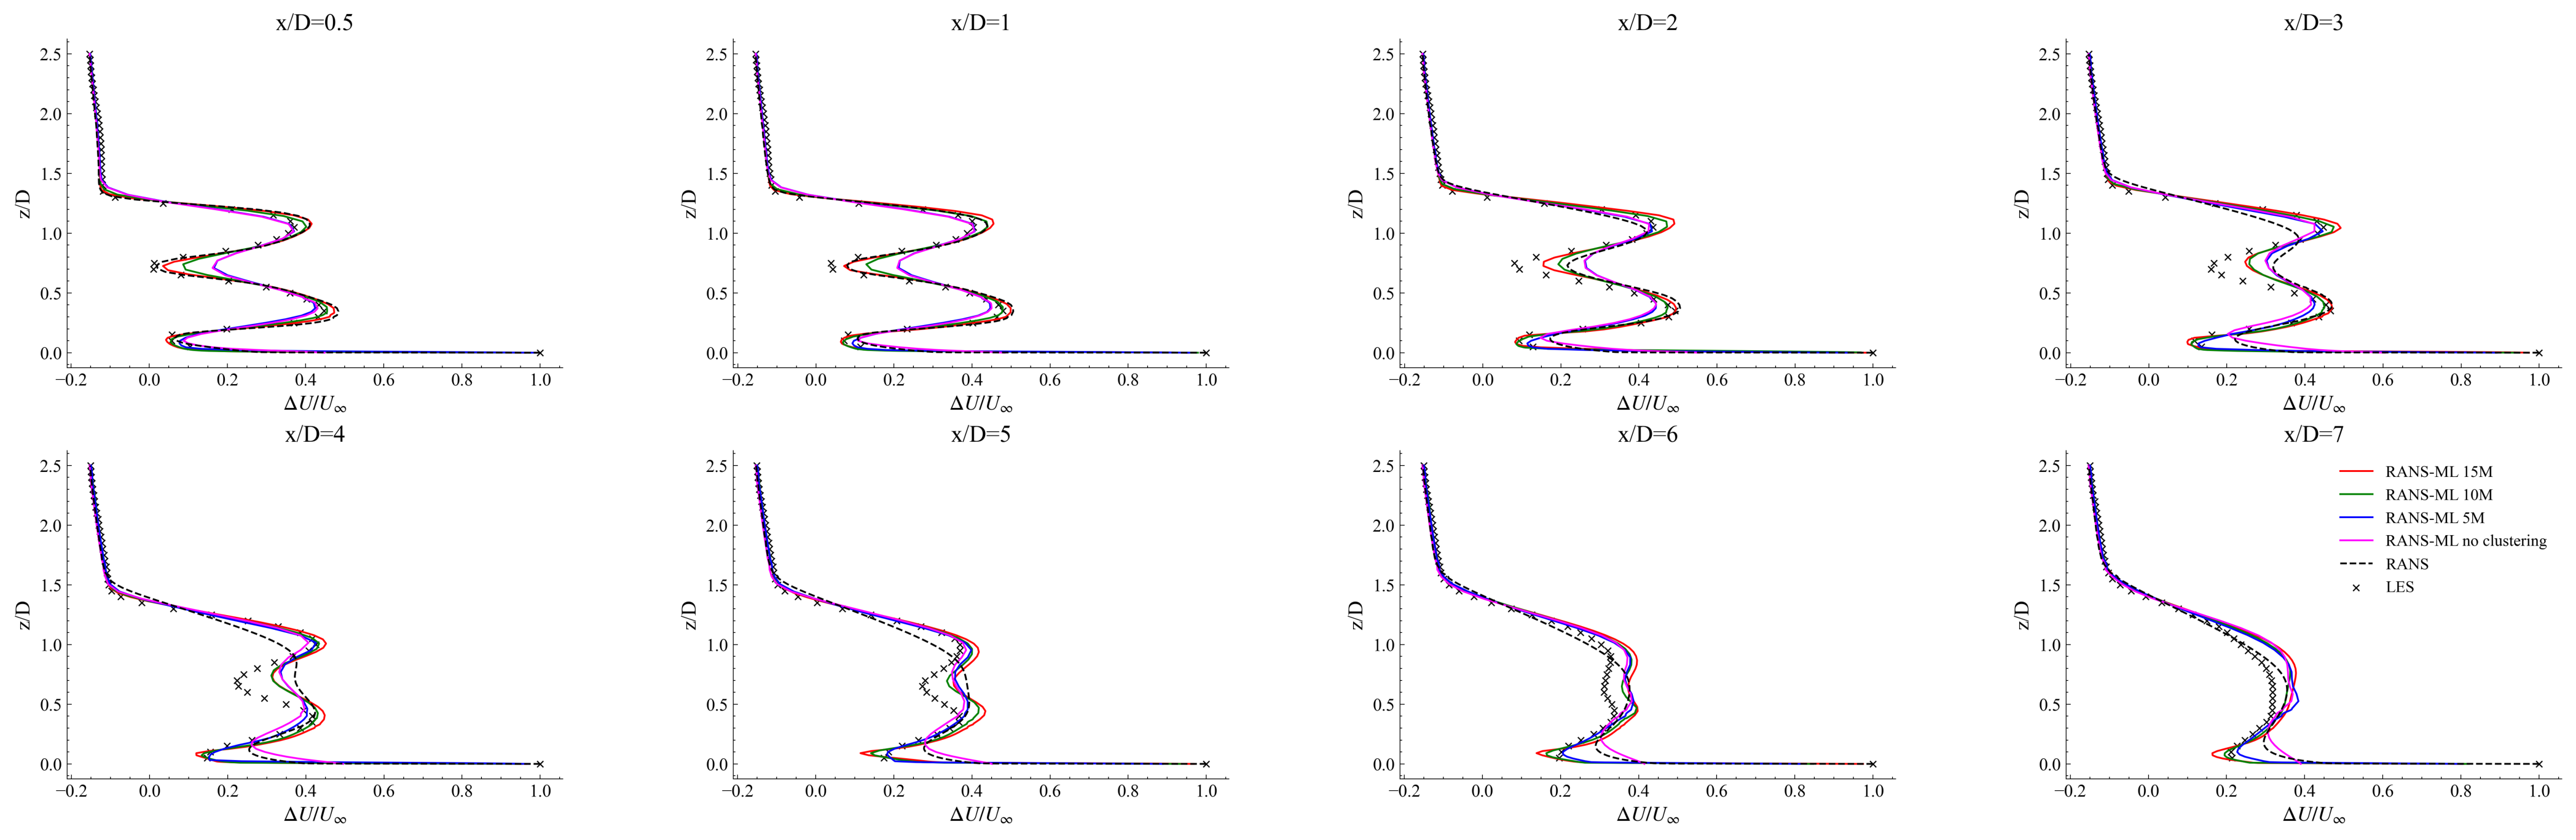
\includegraphics[width=\textwidth]{results/img/ml_results/11ms/deficit/ml_models_comparison/velocity/comparison.png}
        \caption{}
        \label{fig:velocity_deficit_panels}
    \end{subfigure}

    \begin{subfigure}{0.42\textwidth}
        \centering
        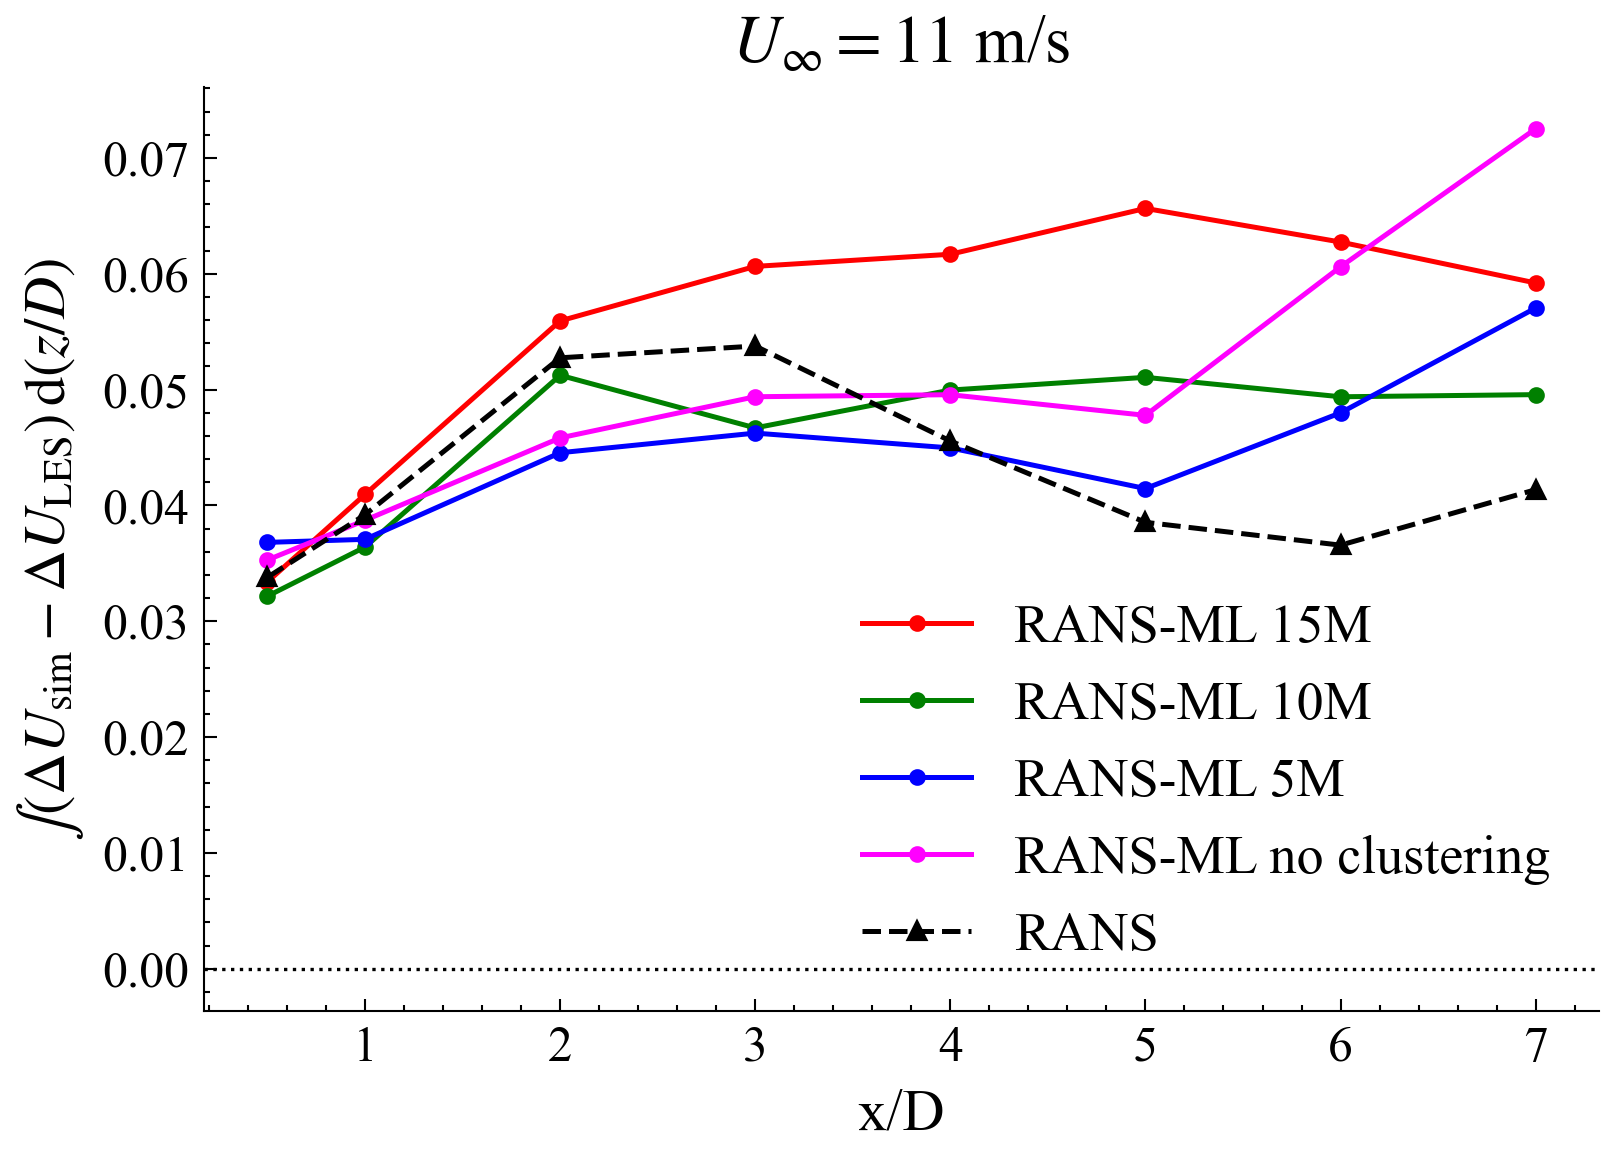
\includegraphics[width=\textwidth]{results/img/ml_results/11ms/integral_deficit_difference.png}
        \caption{}
        \label{fig:velocity_deficit_integral}
    \end{subfigure}
    \caption{Velocity deficit for the 11.4\,m/s inflow condition along the $x$-axis at different streamwise distances
    from the rotor, for the ML-RANS model on grids of different resolution,
    compared with the standard RANS model and the LES reference: (a) deficit profiles at successive
    streamwise stations; (b) signed integral of the velocity-deficit difference with respect to the
    LES reference as a function of the streamwise distance.}
    \label{fig:velocity_deficit}
\end{figure*}

To assess the dynamic effects on the turbine and the associated power production,
the predicted tangential force is reported in
Fig.~\ref{fig:forces} and the $C_p$/$C_t$ coefficients in Tab.~\ref{tab:forces_coeff}. They show good agreement with the reference curves, with a
slight underestimation partly attributable to the fact that the reference refers
to an isolated turbine, whereas the ML-RANS model operates in a turbulent
ABL affected by the ground. Overall, the model reproduces not only the velocity
wake field but also the aerodynamic loading and power production, a key
requirement for wind farm applications.

\begin{table}[t]
    \centering
    \begin{tabular}{l c c}
        \hline
         & ML-RANS & Reference~\cite{NREL_5MW} \\
        \hline
        $C_p$ & 0.448 & 0.490 \\
        $C_t$ & 0.064 & 0.068 \\
        \hline
    \end{tabular}
    \caption{Predicted power ($C_p$) and thrust ($C_t$) coefficients at the reference inflow condition, compared with the reference.}
    \label{tab:forces_coeff}
\end{table}

\begin{figure}[!htb]
    \centering
    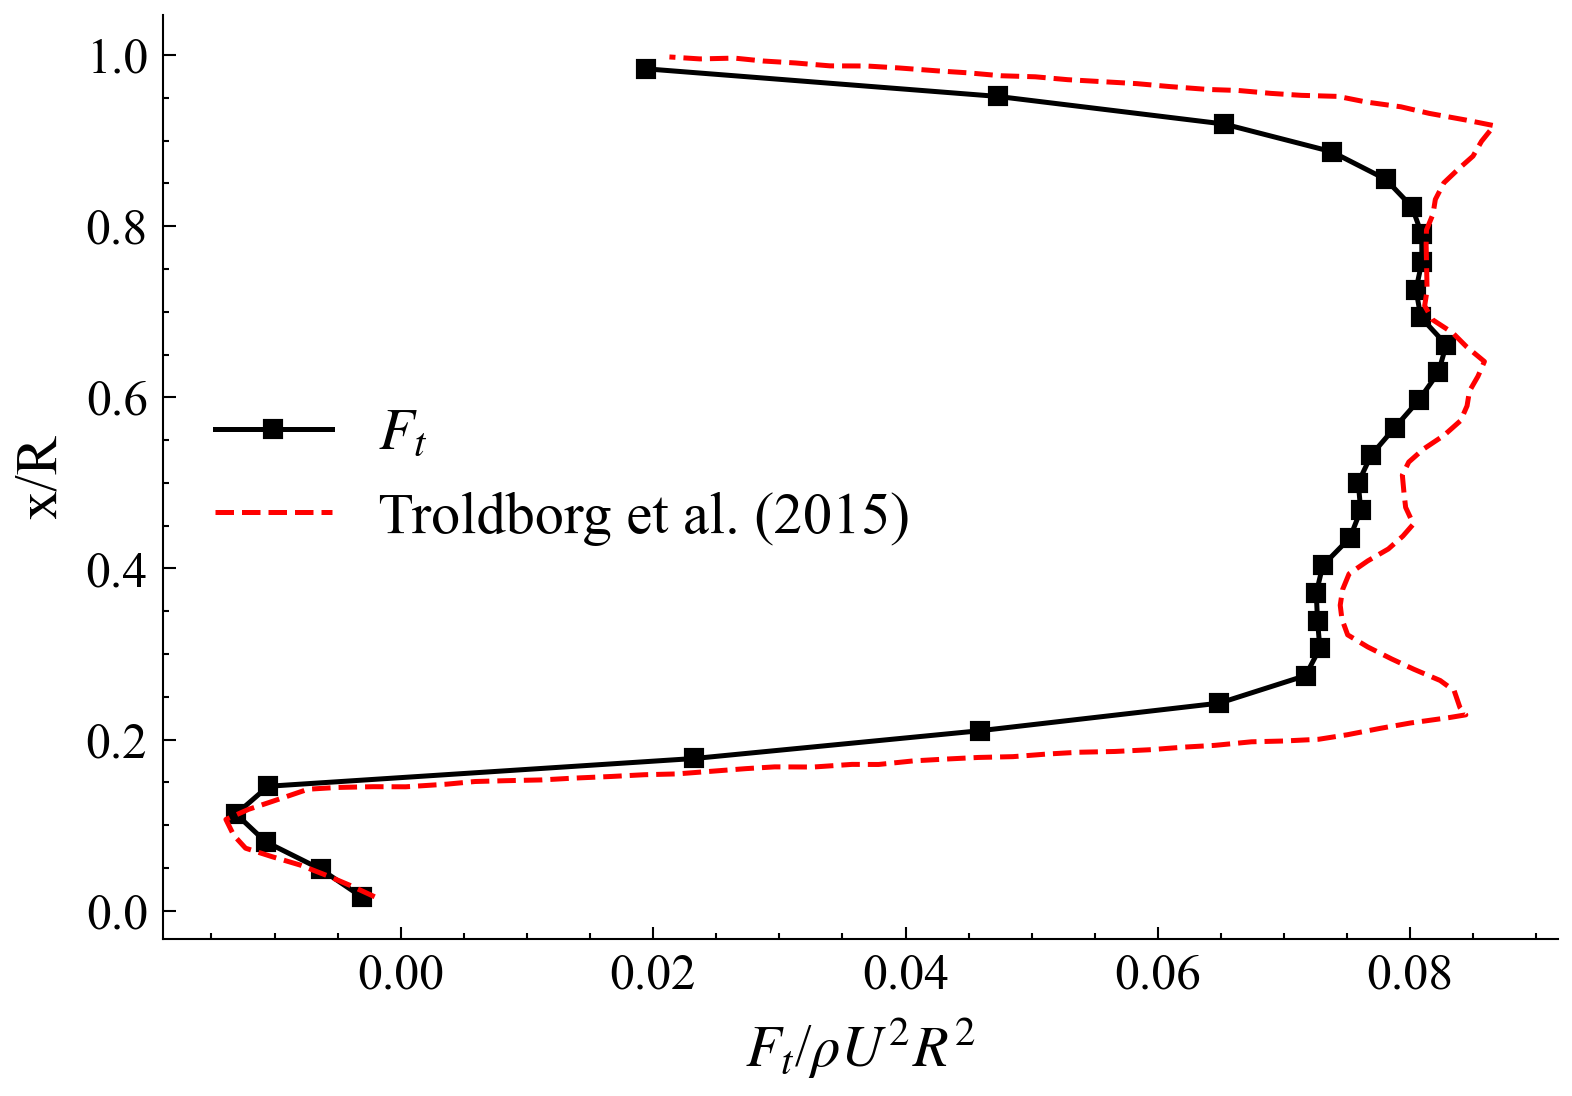
\includegraphics[width=0.45\textwidth]{results/img/forces_profile_tangential.png}
    \caption{Tangential force profile predicted by the ML-RANS model, compared with the reference of Troldborg et al. (2015).}
    \label{fig:forces}
\end{figure}

%%% CONCLUSIONS
\section{Conclusions}
\label{sec:conclusions}
A CFD-ML methodology was presented to build a turbulence closure that improves
the fidelity of RANS simulations of HAWT wakes while keeping the computational
cost compatible with wind farm applications. An LES-equivalent eddy viscosity
extracted from a LES of the NREL-5MW turbine was used as target, a K-means
clustering segmented the domain into seven physically meaningful flow regions,
and an MLP learned the eddy-viscosity correction
$\Delta\nu_t = \nu_{t,eq}-\nu_{t,\mathrm{RANS}}$, embedded into a modified
OpenFOAM PIMPLE solver. The network reproduced the LES-equivalent closure with a
validation $R^2 = 0.9952$, and clustering proved decisive in the near-terrain
region. Once embedded, the ML-RANS model consistently outperformed the
standard RANS model in both near- and far-wake; most notably, on ultra-coarse
grids it accurately reproduced the post-breakdown far-wake recovery at a cost
about $1.25$ times lower than the reference LES, while also reproducing the rotor
forces and $C_p$/$C_t$ coefficients. By design, the closure was calibrated on a single
operating condition and then transferred, without retraining, to coarser grids
and to the unseen $8$ and $15\,\mathrm{m/s}$ conditions, staying close to the LES
throughout: this single-case-to-many transfer is the core contribution of the
work, not a limitation of it. Future work will extend the methodology to multi-turbine configurations, different WT models, towards compact, data-driven closures suitable for real-time wind farm monitoring and control.
Moreover, in future work, the pipeline will be optimised to reduce the inference time of the ML model by avoiding reliance on a Python-based pipeline,which is currently the main bottleneck of the metodology, thereby significantly further reducing computational cost and enabling real-time applications.

%%% BIBLIOGRAPHY
\bibliographystyle{unsrt}
\bibliography{bib/ref.bib}
\end{document}
